\chapter{Experiments}
\label{chap:experiments}

\section{Data Acquisition through Random Motor Babbling}
\label{sec:exp-mb}
The goal of the motor babbling experiment is to simulate the acquisition of hand-eye coordination as it occurs in infants. 
As a result, robot's limb postures achieved in the experiment, characterised through absoulte positions, were stored in a knowledge base.
By equipping the robot with the SOM-based model and using data in the knowledge base we hope to simulate a part of infants' developmental trajectory in an artificial agent. 

The babbling procedure with a random walk strategy has been adapted from 
\citep{SchillaciH11}. Random steps which involve increasing, holding or 
decreasing the joint by angle-step are sampled from a uniform distribution. 
Random steps are iteratively added to the current configuration and the ranges 
of joint configurations in degrees are: for shoulder pitch from -120 to 120, for 
shoulder roll -95 to 0, for elbow roll from 0 to 90 and elbow yaw from -120 to 
120. Only a maximum step of 10 degrees is allowed for each joint. If the 
randomly determined arm position is impossible to reach due to physical 
constraints of the robot's arm, a new position is chosen until the generated 
position is possible. The experiment consisted of a robot randomly babbling with 
its left hand while looking at its own arm movements. Such behaviour consisted 
in the robot moving its arm in a random fashion and generating head movements 
according to the visual perception of its own hand which was tagged with a 
marker. At each time step, which was determined by the capturing rate of the 
camera, positions of the arm were stored in a knowledge base. While the robot 
moves its arm, it estimates the position of its hand by analysing the visual 
input and moves. It moves joints of its neck in order to keep the hand in the 
center of the image. The 3D position of a marker is computed relative to the 
robot torso.

Two babbling experiments were conducted to collect the data. The first experiment lasted for approximately 40 minutes and it yielded 74,143 data points. These data points were used to train the SOM-based models that were implemented on a robot. The second babbling experiment lasted approximately 30 minutes during which 57,778 data samples were collected. This data set was used to check the quality of the model prior to implementation on the robot. The motivation for the quality assessment arose after we tried to use babbling data obtained in a computer simulation for the training of the model. In that case, instead of gathering data via the babbling experiment we used Webots, a software for simulating robots on a computer, to simulate babbling experiment and collect data. When the model trained on this data was implemented on a robot and used in the experiment the pointing was very imprecise. Moreover, the robot's movements appeared almost random disrupting the natural flow of human-robot interaction. The 
reason for this poor performance might have been the lack of noise and ideal conditions imposed by the simulation environment which did not realistically depict the experimental setting. Motivated by the difference between the simulated and the real environment, we decided to perform an additional babbling experiment to check the model performance prior to implementing the model in a robot. 


\section{Model Training}
\label{sec:exp-modtrain}

\subsection{Adjustment of Weights}
The training of the model consisted of two phases. In the first phase, only the 
local neural weights in each SOM were adjusted. In total, there were 20,000 
iterations in which an input vector was randomly chosen from a babbling 
knowledge base gathered in the first babbling experiment. The input vector was 
a 7D vector, which was divided into the 3D hand vector and the 4D joint vector. 
The hand vector was presented to the first SOM and the 4D joint vector to the 
second SOM. Winning neurons in both SOMs were detected as the ones with the 
lowest Euclidean distance to the input vector. Weights of winning neurons and 
neurons surrounding them were adjusted according to the formulas explained in 
the section \ref{sec:sommath}.
In the second phase, the winning neurons in both SOMs were associated using the Hebbian learning rule which defined the connection strength based on their level of activation.

\subsection{Training Parameters}
The learning rate $\eta$ was set to 0.9 and the spread of the Gaussian neighbourhood function $\sigma$ was 0.7. Both hyperparameters were kept constant for the first half of iterations, and afterwards annealed exponentially. The scaling factor used to associate neurons between the two SOMs, $\eta_h$ was set to a constant value 0.01 ensuring the positive weight growth.\\

\subsection{Model Configurations}
We trained three different instances of a model: the $5\times 5$ model consisted of two 2D SOMs with each SOM having 25 neurons, the $10\times 10$ model consisted of two 2D SOMs with each SOM having 100 neurons and the $15\times 15$ model with 225 neurons in each SOM. In addition, we investigated the influence of the training data on all three models and present the results in the following section. In the same section we tested all three models using the second babbling data set to measure pointing accuracy.
The $5\times 5$ and the $15\times 15$ model were implemented on the humanoid robot and used in an experiment with a human. The SOM covering the hand space from the $5\times 5$ model is shown in Figure \ref{lab:5x5} and the same SOM from the $15\times 15$ model is shown in Figure \ref{lab:15x15}. 
The motivation for investigating models of different sizes comes from the assumption that bigger networks might evolve from the smaller ones. In this way, the progression of skill development is followed by the increased number of neurons specialized in coding od sensorimotor experience. All models were trained using the same parameters.

\begin{figure}[t]
\centering
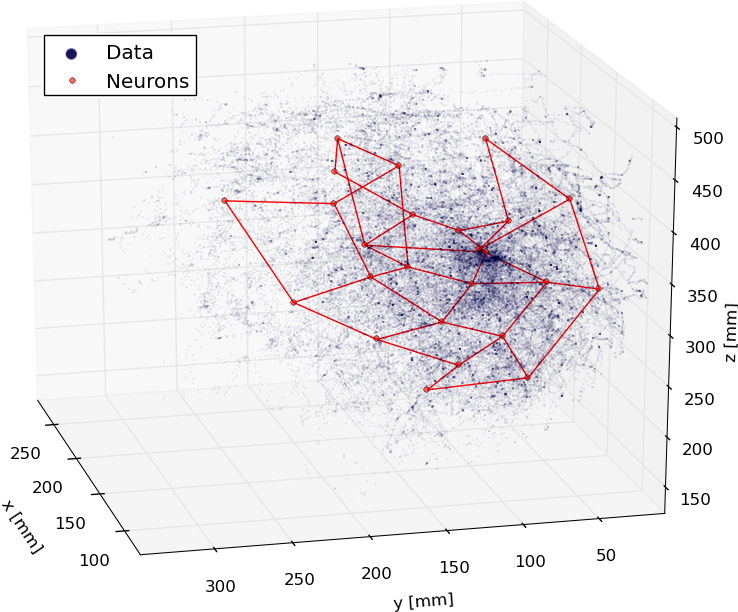
\includegraphics[scale=0.55]{SOM_5x5.png}
%\epsfig{file=SOM_5x5_zoom.png}

\caption{The SOM with 25 neurons approximating the left hand trajectory samples in the \ssom model}
\label{lab:5x5}
\end{figure}

\begin{figure}[t]
\centering
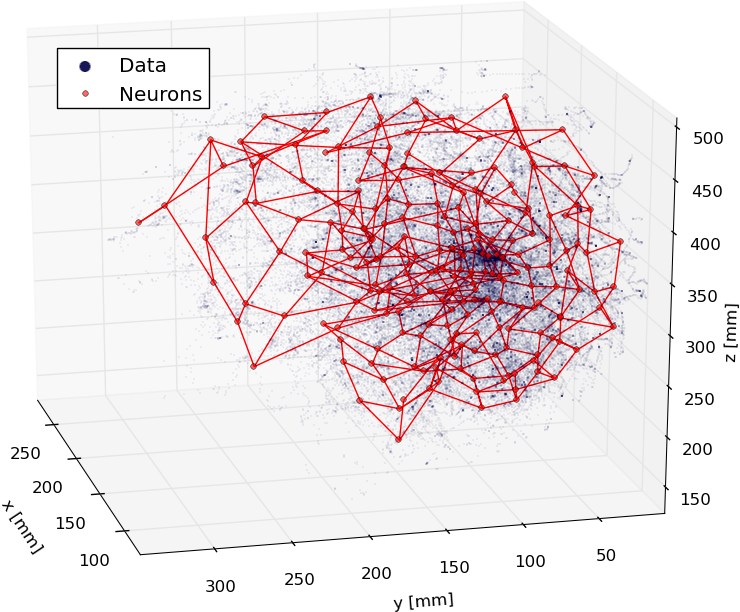
\includegraphics[scale=0.55]{SOM_15x15.png}
\caption{The SOM with 225 neurons approximating the left hand trajectory samples in the \bsom model}
\label{lab:15x15}
\end{figure}

% \begin{figure}[h]
% \centering
% \epsfig{file=hebb.png, height=6cm}
% \caption{Hebbian weights}
% \label{lab:5x5}
% \end{figure}


\section{Preliminary Results}
The goal of preliminary computational experiments is to investigate the quality of models prior to the implementation on a robot. This is a sanity check that ensures there are no errors or bugs in the program that might be hard to detect once the model is implemented on the robot.
First, we trained the three models on the the data gathered in the first babbling experiment. Second, we altered the training procedure in two ways: either by picking only the first $p$ fraction of the points from the babbling session, simulating a shorter babbling phase, or by picking every $n$th data point, thus simulating a babbling process that was slightly ``sped-up''. All models were tested only using the data points from the second babbling experiment.

The testing procedure comprised of presentation of a 3D hand vector to the first SOM, activating a winning node and computing the Euclidean distance between them. In table \ref{lab:table_trainf} we present errors for all models that were trained on different amounts of data, but where training data points were picked uniformly such that each $n$th point was chosen.

\renewcommand{\arraystretch}{1.5}
\begin{table}[t]\footnotesize
\begin{center} 
 \caption{Errors for all three models and training sets using approximately first $p$ percent of training data}
 \label{lab:table_trainf}
 \begin{tabular}{|c|c|c|c|}
   \hline     
    p= & $1\%$ data & $10\%$ data & $100\%$ data\\ \hline
   $5\times 5$ & $46.00 \pm 37.75$ & $29.82 \pm 18.15$ & $29.11 \pm 14.99$ \\ \hline
   $10\times 10$ & $39.65 \pm 37.96$ & $21.44 \pm 17.22$ & $18.87 \pm 11.68$ \\ \hline
   $15\times 15$ & $39.45 \pm 38.23$  & $17.82 \pm 15.78$ & $14.18\pm 8.30$ \\  
   \hline
 \end{tabular}
\end{center}
\end{table}

We see that the increase in number of neurons is followed by the lower error and that  models trained on more data perform better. From computational point of view this result is expected as more neurons provide higher resolution of the input space. However
In table \ref{lab:table_trainu}, we show the three models trained on different amounts of data where training points were used only from the beginning of the babbling set.

\renewcommand{\arraystretch}{1.5}
\begin{table}[h]\footnotesize
\begin{center} 
 \caption{Errors for all models and training sets using every $n$-th data point}
 \label{lab:table_trainu}
 \begin{tabular}{|c|c|c|c|}
   \hline     
    n= & $100$ ($1\%$ data) & $10$ ($10\%$ data)\\ \hline
   $5\times 5$ & $29.48 \pm 15.98$ & $28.92 \pm 14.45$  \\ \hline
   $10\times 10$ & $18.66 \pm 11.48$ & $18.43 \pm 10.29$ \\ \hline
   $15\times 15$ & $14.33 \pm 9.03$  & $13.90 \pm 7.95$\\  
   \hline
 \end{tabular}
\end{center}
\end{table}

As expected, if training points were chosen randomly from the whole babbling set compared only to the first $n$ points, the errors were much lower. 
In addition it is interesting to notice that models trained only on 1\% (cca. 700 data points) of the randomly chosen training data were performing just slightly worse (or approximately equal) than the models trained on the 100\% of the data. 

\section{Human-Robot Interaction}
\label{sec:exp-hri}

\begin{figure}[h]
\centering
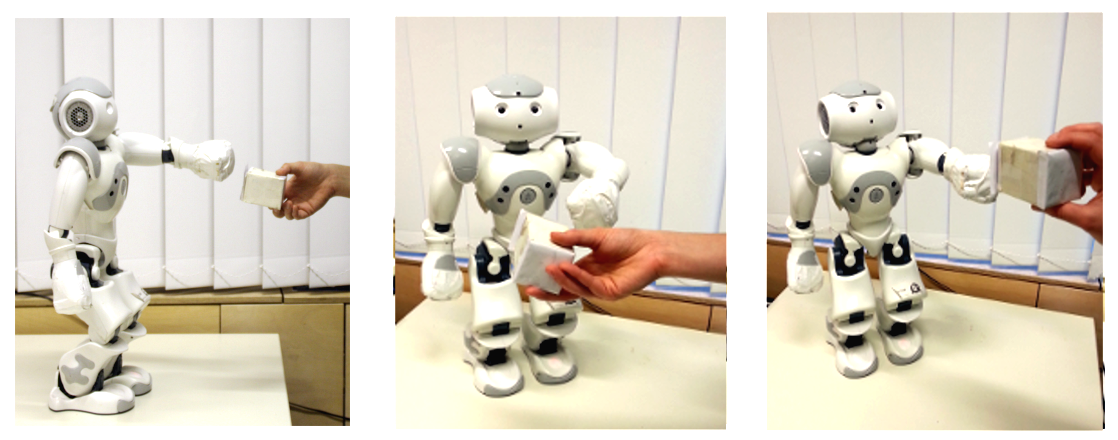
\epsfig{file=experiment_new.png, height=5cm}
\caption{Pointing sequence in a human-robot interaction}
\label{lab:experiment}
\end{figure}

Both the \bsom and \ssom models trained on data acquired in the babbling experiment were implemented on a robot. The robot equipped with models was standing in front of a human subject on a table as shown in Figure \ref{lab:experiment}. The experimenter held an object tagged with a marker and moved it randomly within the visual field of the robot. The movements were performed at a varying speed, trying not to exceed the speed of the robot's moving hand. The experimenter tried to cover the space within and beyond the reach of the robot's hand to explore the extend of possible arm configurations. While the object was moved in front of the robot, it followed the marker with its arm and gaze. For positions within the reach of its hand, the robot bended the arm to point to the object. For positions beyond the reach of its hand, the robot extended the arm in the direction of the object. This action was interpreted as pointing. The experiment took place for approximately 2.5 minutes and the arm position 
characterised through hand and joint coordinates was stored every 100 ms on a memory disk in the robot. As seen in the 
figure, the problem of various arm configurations resulting in the same hand positions was successfully resolved using the SOM-based model.

In the experiment with a human subject, the \bsom model was used to determine the left arm position at every time step a marker was detected. The procedure to determine the arm configuration was following. First, the robot detected 3D marker coordinates using the camera in its head. Marker coordinates were described as a 3D vector containing the horizontal, the vertical and the depth dimension ($\mathbf{w_m}$). 
The 3D vector was presented to the first SOM and a winning neuron $\mathbf{w_i}$ was selected such that: 
\begin{equation}
\underset{i}{\arg\min} \hspace{1mm} ||\mathbf{w_m}-\mathbf{w_i} ||
\end{equation}

Based on the strongest Hebbian connection from the winning neuron $i$ in the first SOM, a neuron $j$ in the second SOM was selected such that: 
\begin{equation}
\underset{j}{\arg\max} \hspace{1mm} w_{hebb}(i, j) 
\end{equation}

$w_{hebb}$ denotes Hebbian weights estimated in the training process.
Weights of a winning neuron ($\sigma_p, \sigma_r, \epsilon_y, \epsilon_r$) in the second SOM were used to issue the motor command to set arm joints. The first two dimensions of a weight vector ($\sigma_p, \sigma_r$) were used to set the shoulder pitch and shoulder roll, and the two second dimensions ($\epsilon_y, \epsilon_r$) to set the elbow yaw and elbow row. Concurrently to the activation of a winning neuron in the second SOM of a \bsom model, the winning neuron in the second SOM of a \ssom model was detected. The procedure was the same for both models, but the weights of a winning neuron in the \ssom model were not used to steer arm kinematics. They were stored and used for comparison between the object position, and the winning weights of the \bsom model.


